\documentclass[a4paper,12pt]{article}
\usepackage{pdfpages}
\usepackage{graphicx}

\title{Training village PCBs documentation}
\date{2026-03-03}
\begin{document}
\maketitle
\pagenumbering{gobble}
\newpage

\pagenumbering{arabic}
\section{Introduction}

The system is comprised of three boards. The main one is a raspberry pi shield, seen in fig \ref{fig:rpishield}, which exposes three ethernet connectors that go to the other two boards. It also features a DC connector to power the servos and other peripherals. 

\begin{figure}[htbp] % Placement options: h=here, t=top, b=bottom, p=page of floats
  \centering % Center the figure
  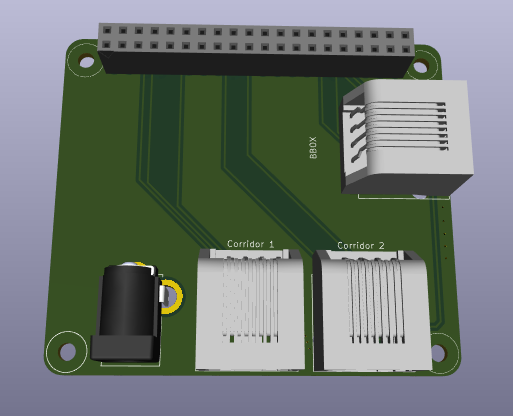
\includegraphics[width=0.6\textwidth]{RPiShield.png} % Include image (no extension needed usually)
  \caption{3D render of the Raspberry Pi shield.}
  \label{fig:rpishield} % Label for cross-referencing
\end{figure}

To control the corridor a PCB is designed, this board has connectors to control the motors, the LED strip, the 

\begin{figure}[htbp] % Placement options: h=here, t=top, b=bottom, p=page of floats
  \centering % Center the figure
  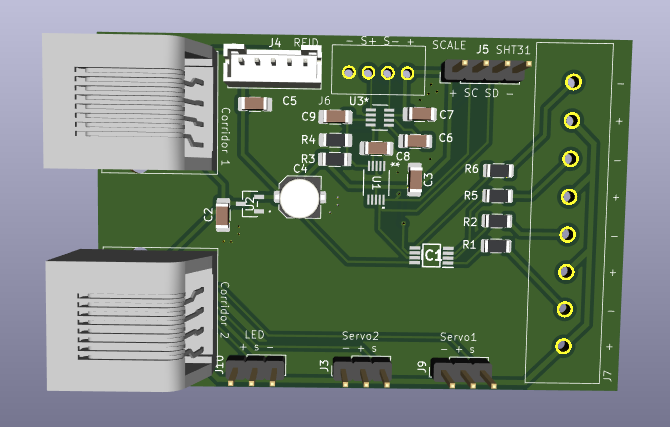
\includegraphics[width=0.6\textwidth]{Corridor.png} % Include image (no extension needed usually)
  \caption{3D render of the corridor PCB.}
  \label{fig:corridor} % Label for cross-referencing
\end{figure}

The behaviour box is controlled from another board that features one connector for a servo and two connectors for LED strips. This board also allows to connect IR LEDs with a screwed connector.

\begin{figure}[htbp] % Placement options: h=here, t=top, b=bottom, p=page of floats
  \centering % Center the figure
  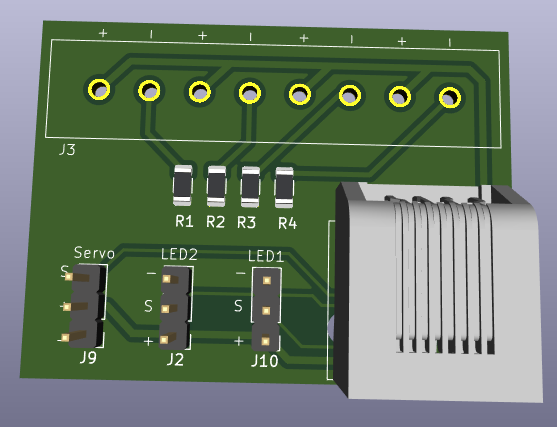
\includegraphics[width=0.6\textwidth]{BBOX.png} % Include image (no extension needed usually)
  \caption{3D render of the behaviour box PCB.}
  \label{fig:BBOX} % Label for cross-referencing
\end{figure}



\newpage

\section{Absolute maximum ratings}

Here is presented a table that summarizes the absolute maximum rating of the system.

\begin{table}[htbp] \centering
    \begin{tabular}{l|l|l}
        \emph{Parameter} & \emph{Value} & \emph{Units}\\ \hline
        Input DC jack voltage & 0-6 & V\\
        Output current & 1 & A
    \end{tabular}
\caption{Absolute maximum ratings table}\label{tab:exp}
\end{table}
\newpage

\section{Annex}
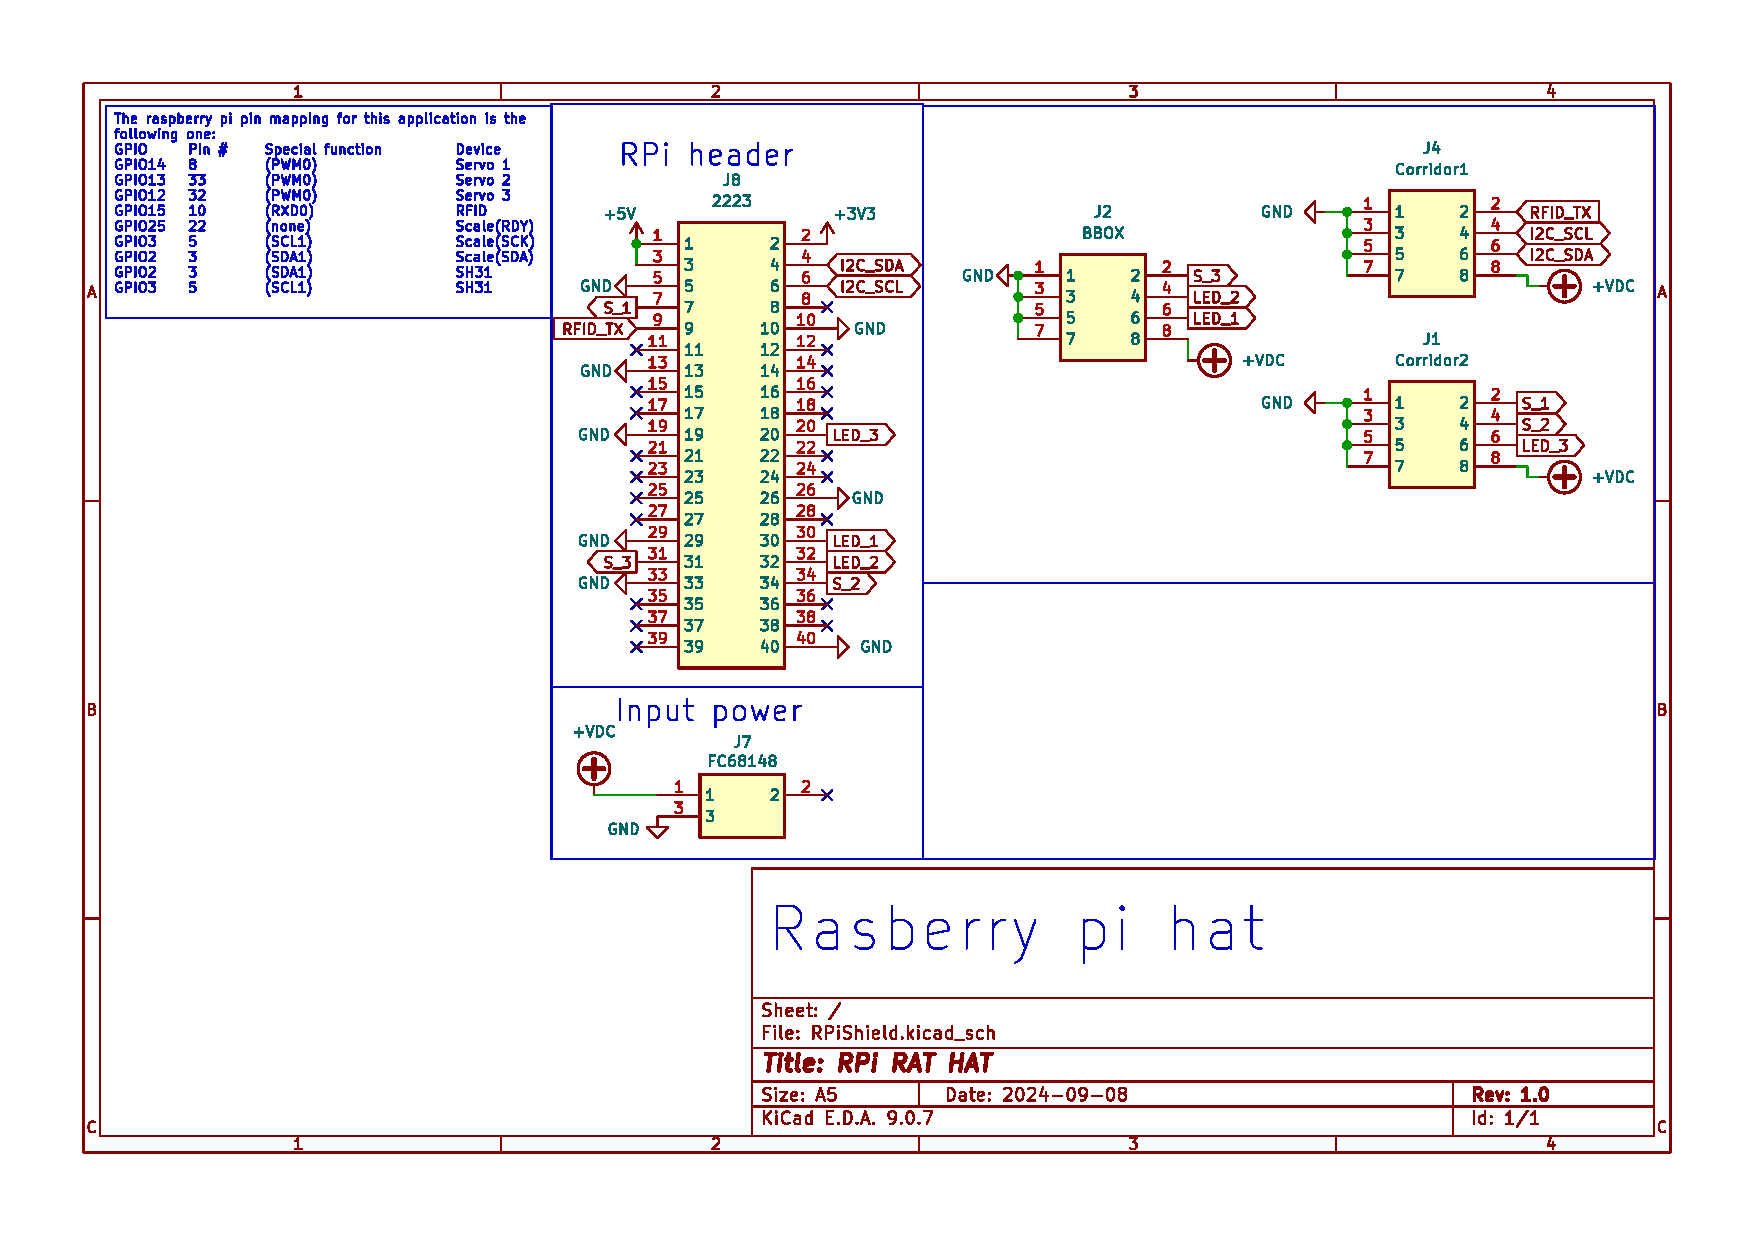
\includepdf[]{RPiShield.pdf}
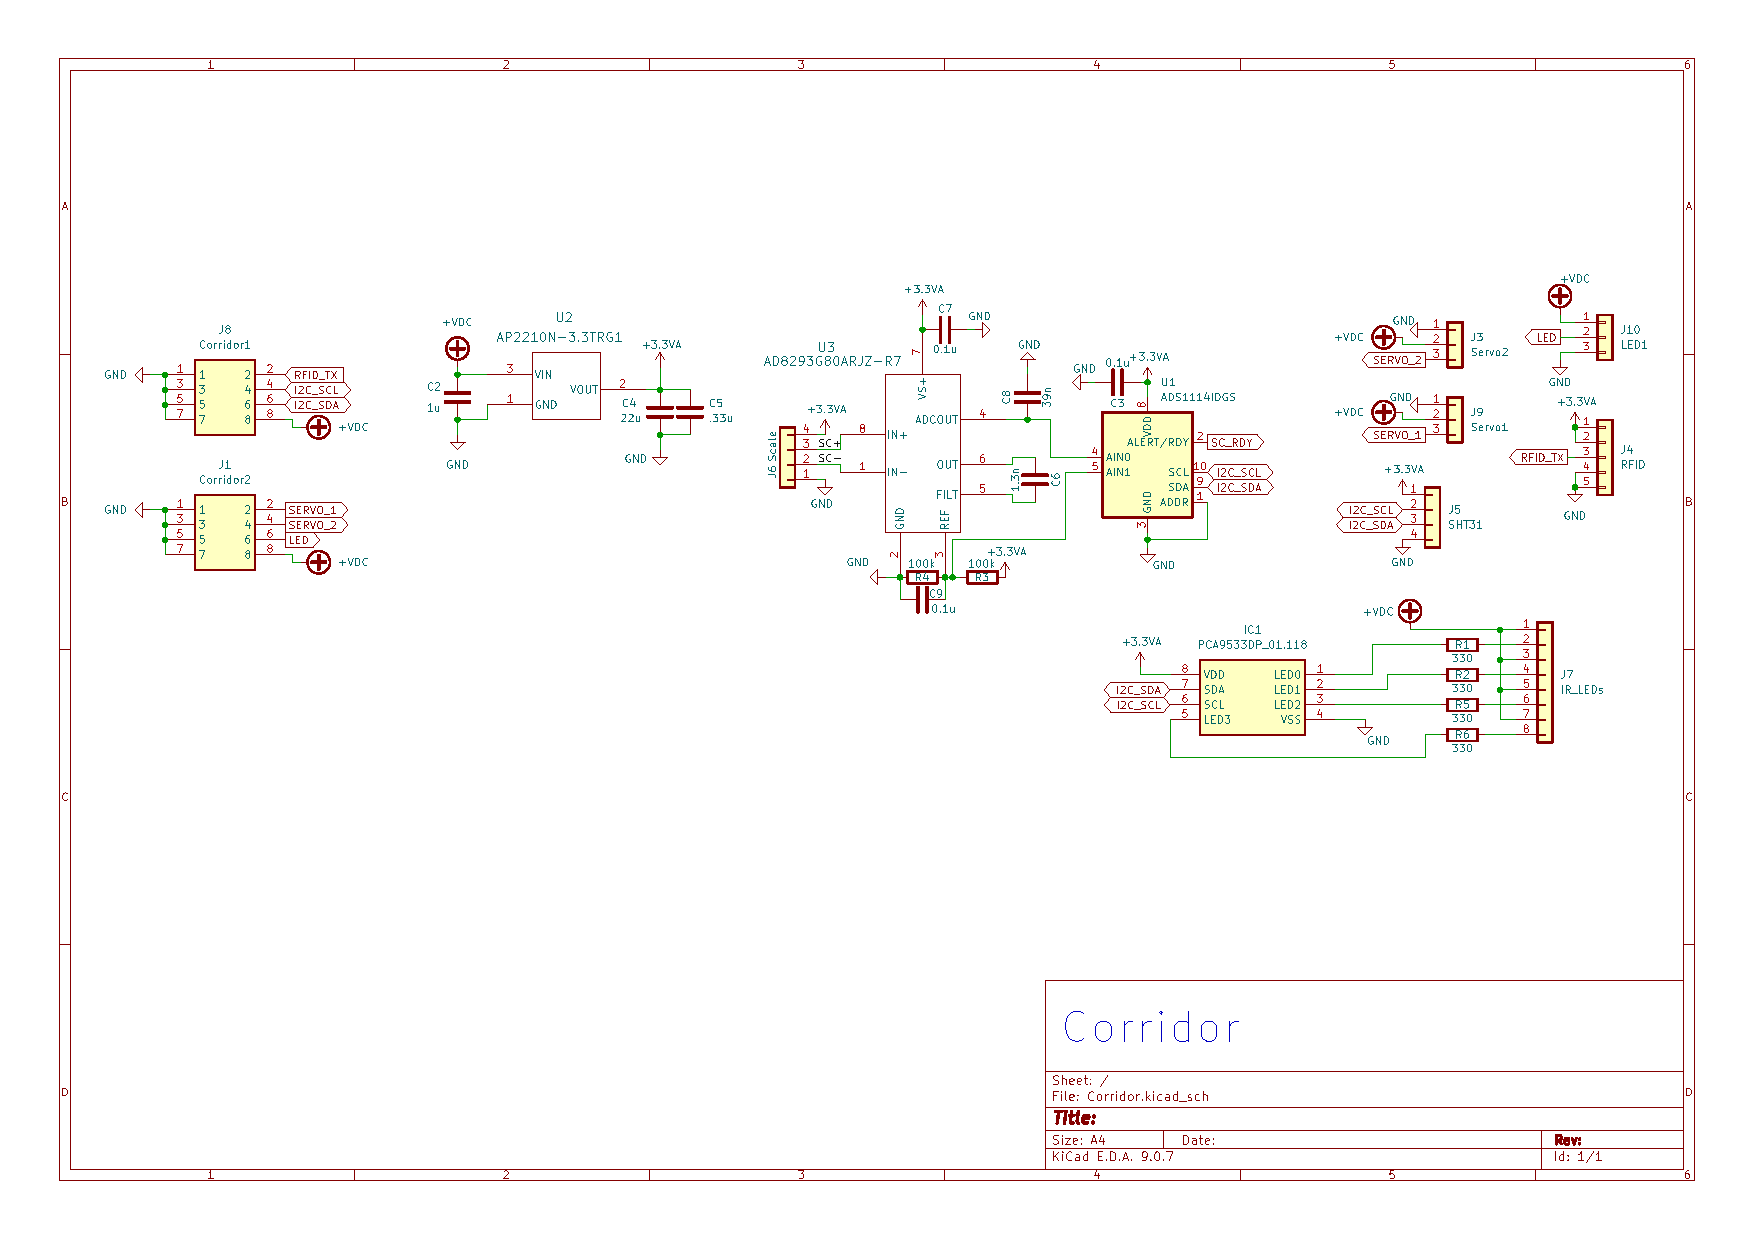
\includepdf[]{Corridor.pdf}
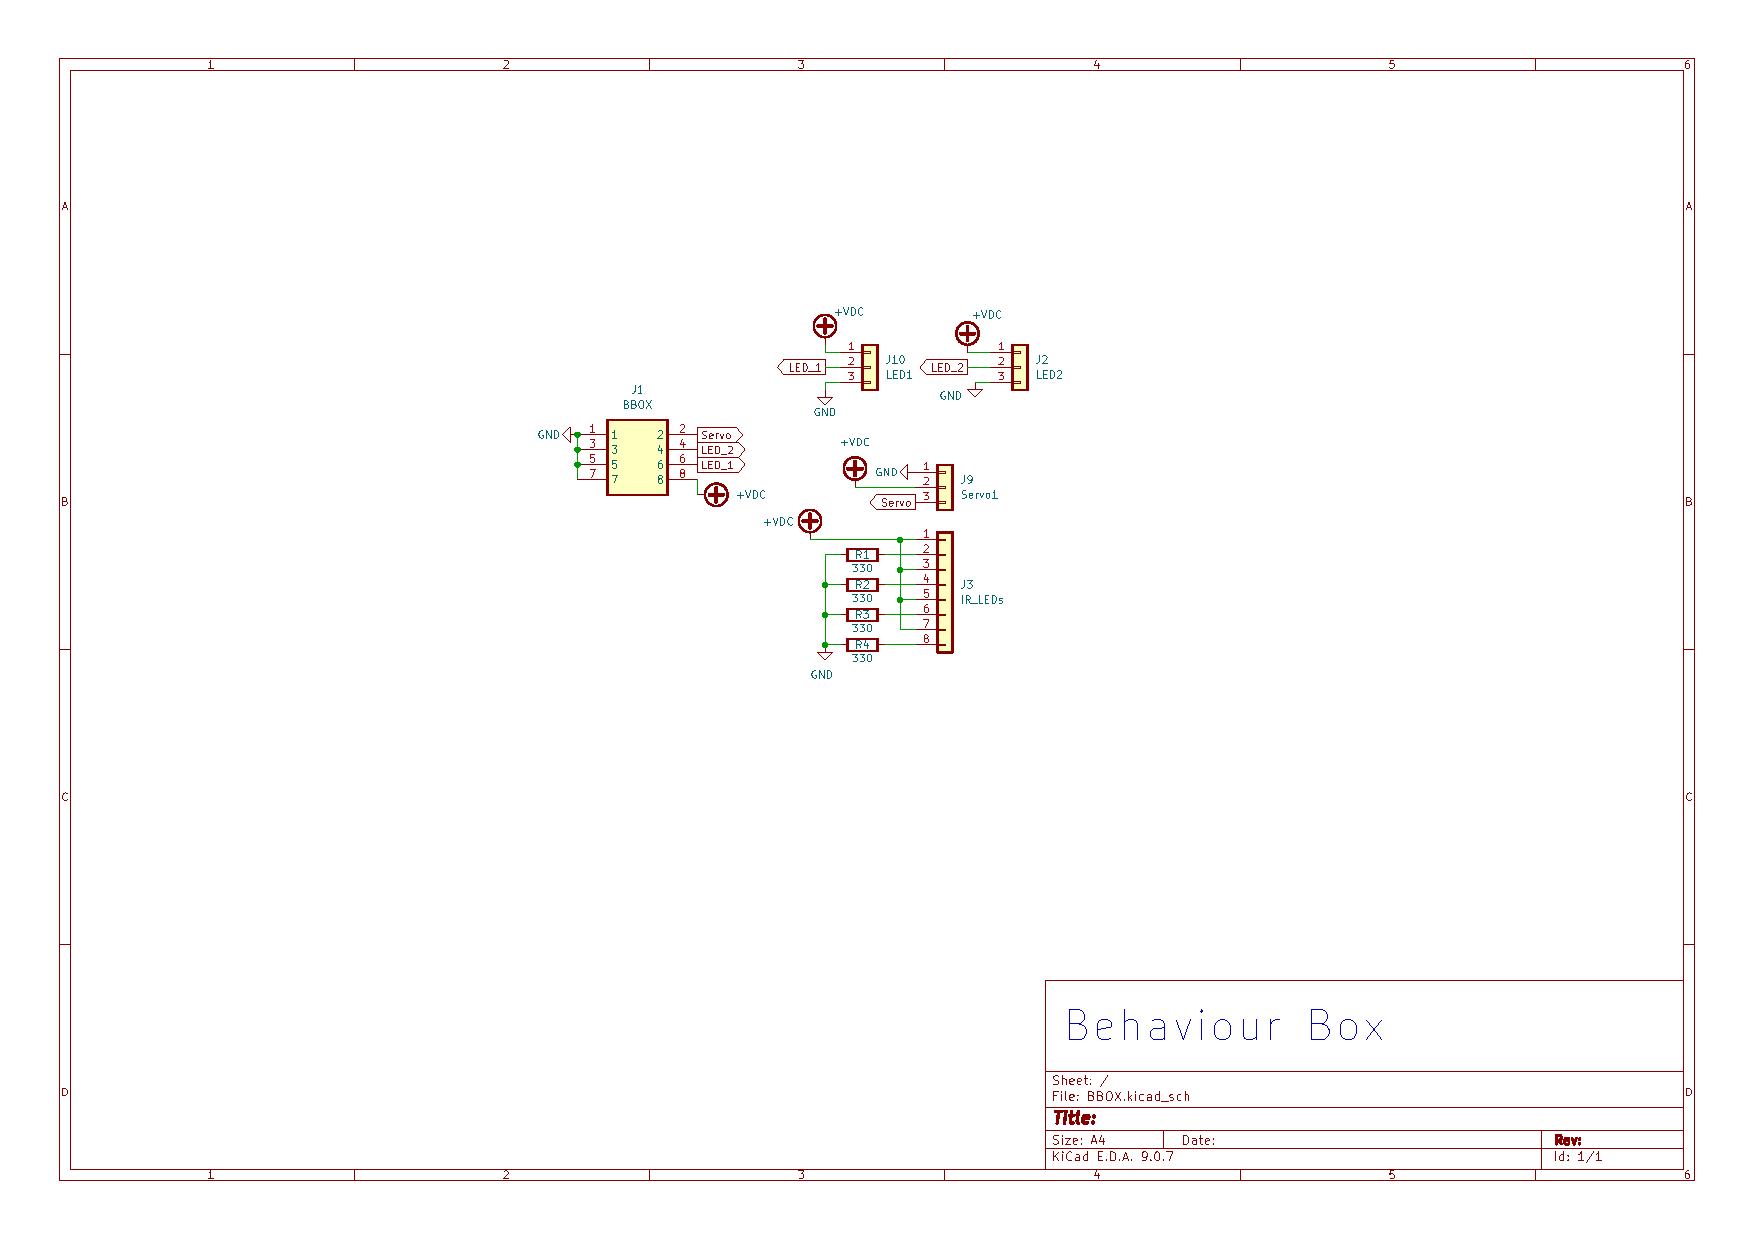
\includepdf[]{BBOX.pdf}
\end{document}